\chapter{Finite Element Methods}

In this chapter, we will cover the basics of the theory of finite element methods. 

\section{Basics and Notations}
For convenience in notation for partial derivatives, we introduce the following notation using the multi-index.

\begin{definition}[Definition of multi-index]
	Let $ n \in \N $. Then the following $m$-tuple
	\[ \alpha = (\alpha_1,\alpha_2,\cdots,\alpha_n) \in \R^n \]
	is called a multi-index, with its length defined as
	\[ \abs{\alpha} = \alpha_1 + \alpha_2 + \cdots + \alpha_n \]
\end{definition}

Now we can have a very compact notation for the partial derivatives of a function using the notion of multi-index.

\begin{definition}[Partial derivatives with multi-index]
	Let $ \Omega \subset \R^n $, and $ f:\Omega \to \R $ be $ m $-times continuously differentiable. Then we have
	\[ D^\alpha f = \big( \frac{\partial}{\partial x_1} \big)^{\alpha_1} \big( \frac{\partial}{\partial x_2} \big)^{\alpha_2}  \cdots \big( \frac{\partial}{\partial x_n} \big)^{\alpha_n}f = \frac{\partial^{\abs{\alpha}}}{\partial x_1^{\alpha_1}\ \partial x_2^{\alpha_2}\ \cdots \partial x_n^{\alpha_n}} f. \]
	Note that since the function is $ m $-times differentiable, then the above definition is defined for $ \abs{\alpha} < m $.
\end{definition}

\begin{example}
	Suppose that $ n=3 $, and $ \Omega \subset \R^3 $. Define $ f: \Omega \to \R $. Then we have
	\begin{align*}
		\sum_{\abs{\alpha}=3} D^{\alpha} f &=  (\frac{\partial^3}{\partial x_1^{3}} + \frac{\partial^3}{\partial x_2^{3}} + \frac{\partial^3}{\partial x_3^{3}} + \frac{\partial^3}{\partial x_1^{2}\partial x_2^{1}} + \frac{\partial^3}{\partial x_1^{1}\partial x_2^{2}} + \frac{\partial^3}{\partial x_2^{1}\partial x_3^{2}} + \frac{\partial^3}{\partial x_2^{2}\partial x_3^{1}} \\
		&+ \frac{\partial^3}{\partial x_1^{1}\partial x_3^{2}} + \frac{\partial^3}{\partial x_1^{2}\partial x_3^{1}} + \frac{\partial^3}{\partial x_1^{1}\partial x_2^{1}\partial x_3^{1}})f.
	\end{align*}
	This example shows how we can simply avoid writing 10 terms using a appropriately designed notation.
\end{example}

\subsection{Space of Continuously Differentiable Functions}

Now we review some basic definitions about the function spaces.
\begin{definition}[Space of continuous functions]
	Let $ \Omega \subset \R^n $, an open region. The space of all continuous functions defined on this region is denoted by $ \mathscr{C}^0(\Omega) $ and defined as follows
	\[ \mathscr{C}^0(\Omega) = \Set{f:\Omega\to \R \ :\ f \text{ is continuous}}. \]
	Also, let $ \mathscr{C}^0(\closure{\Omega})$ denote the set of all functions $ f\in \mathscr{C}^0(\closure{\Omega}) $ that can be extended from $ \Omega $ to a continuous function defined on $ \closure{\Omega} $.\\
\end{definition}
\begin{remark}
	Note that since $ \closure{\Omega} $ compact, then all of the functions in $ \mathscr{C}^0(\closure{\Omega}) $ are bounded. That is true because all the continuous functions defined on a compact set are uniformally continuous, thus bounded.
\end{remark}

\begin{example}
	Let $ \Omega = (0,1) $. Then $ f: \Omega \to \R $, where $ f(x) = 1/x $ is in $ \mathscr{C}^0(\Omega) $ but not in $ \mathscr{C}^0(\closure{\Omega}) $. I.e.
	\[ f \in \mathscr{C}^0(\Omega), \qquad f\notin \mathscr{C}^0(\closure{\Omega}). \]
\end{example}


\begin{proposition}[Vector space structure of the space of continuous functions]
	Let $ \Omega \subset \R^n $. The space $ \mathscr{C}^0(\Omega) $ is a vector space. A suitable norm for this space is defined as follows
	\[ \norm{f} = \norm{f}_\infty = \sup_{x\in \Omega}\abs{f(X)},\]
	where $ f \in \mathscr{C}^0(\Omega) $.
\end{proposition}

\begin{lemma}
	Let $ f \in \mathscr{C}^0(\closure{\Omega}) $. Then
	\[ \norm{f}_\infty = \sup_{x\in \Omega}\abs{f(x)} = \max_{x\in \Omega}\abs{f(x)}. \]
\end{lemma}
\begin{proof}
	A continuous function defined on a compact set attains its maximum and minimum in the set. 
\end{proof}
Now we can define the space of $ k $-times continuously differentiable functions. 

\begin{definition}[The space of k-times continuously differentiable functions]
	Let $ \Omega \subset \R^n $. Then we define the space of $ k $-times continuously differentiable functions defined on $ \Omega $ as 
	\[ \mathscr{C}^k(\Omega) = \Set{f \in \mathscr{C}^0(\Omega)\ :\ D^\alpha f \in \mathscr{C}^0(\Omega) \quad \text{for}\ \abs{\alpha} \leq k   }. \]
\end{definition}

Similar to the space of all continuous functions, the space of all $ k $-times continuously differentiable functions also has a vector space structure as reflected by the following lemma.

\begin{lemma}
	Let $ \Omega \subset \R^n $. Then $ \mathscr{C}^k(\Omega) $ is a vector space. The following norm is a useful norm for this space. 
	\[  \norm{f}_{\mathscr{C}^k} = \sum_{\abs{\alpha} \leq k} \norm{D^\alpha f}_\infty. \]
\end{lemma}
\begin{remark}
	We can of course come up with many other norms, some of them as good as the norm defined above. 
	\[ \norm{f}_{\mathscr{C}^k} = \big(\sum_{\abs{\alpha} \leq k} \norm{D^\alpha f}^p_\infty \big)^{1/p}. \]
	And if we let $ p \to \infty $ then 
	\[ \norm{f}_{\mathscr{C}^k} = \sup_{\abs{\alpha}\leq k} \norm{D^\alpha f}_\infty = \max_{\abs{\alpha}\leq k} \norm{D^\alpha f}_\infty. \]
	Note that we say these norms are good in a sense that it makes the space of interest a complete normed vector space, i.e. a Banach space. 
\end{remark}

\begin{observation}
	Considering the remark above, $ \mathscr{C}^k(\Omega) $ kind of resembles the Euclidean space $ \R^n $ in the sense of extending a norm from $ \R $ to $ \R^k $.
\end{observation}

The following example demonstrates all of these definitions in a more concrete example.

\begin{example}
	Let $ \Omega \subset \R^2 $, open and bounded. The the space of all one time continuously differentiable functions is
	\[ \mathscr{C}^1(\Omega) = \Set{f\in \mathscr{C}^0(\Omega)\ :\ \partial_{x}f \in \mathscr{C}^0(\Omega)\ \text{and}\ \partial_y f \in \mathscr{C}^0(\Omega)}. \]
	And the corresponding suitable norm for this space is
	\[ \norm{f}_{\mathscr{C}^k} = \norm{f}_\infty  + \norm{\frac{\partial f}{\partial x}}_\infty + \norm{\frac{\partial f}{\partial y}}_\infty. \]
\end{example}

\subsection{Space of Lebesgue Integrable Functions}
Here, we define some spaces of functions that are basically characterizing the growth and decay rate of functions. The following definition makes this more clear. 
\begin{definition}
	Let $ \Omega \subset \R^n $, and let $ p\geq 1 $ be a real number. Then we define
	\[ \tilde{L}_p(\Omega) = \Set{f:\Omega\to\R\ :\ \big(\int_\Omega \abs{f(x)}^p dx \big)^{1/p} < \infty} \]
\end{definition}

The following proposition is very crucial for our up coming discussions.
\begin{proposition}
	Let $ \Omega \subset \R^n $, and $ p\geq 1 $. Then $ (\tilde{L}_p(\Omega)/\!\!\sim, \norm{\cdot}_{L_p}) $ is a normed vector space, where $ \sim $ is a equivalence relation defined on the set $ L_p(\Omega) $ identifying the functions that are equal almost everywhere. Further more the norm is defined as
	\[ \norm{f}_{L_p} = \big(\int_\Omega \abs{f(x)}^p dx\big)^{1/p}.\]
	We denote 
	\[  L_p(\Omega) :=  \tilde{L}_p(\Omega)/\!\!\sim \]
\end{proposition}
\begin{remark}
	There are some notes to emphasis here. \\
	1. We defined the $ L_p(\Omega) $ to be the quotient set $ \tilde{L}_p(\Omega)/\!\!\sim  $. The reason for that is because the $ \norm{\cdot}_{L^p} $, when defined on $\tilde{L}_p$ is no longer a norm, as it is not positive definite. I.e., the norm of a function in $ \tilde{L_p} $ can be zero, while the function is not identically zero, but is zero almost everywhere, i.e. on a set of measure zero. That is why we need to identify the functions that are equal almost everywhere. \\
	2. To check to see see if the norm defined as above satisfies the properties of norm, we can use the Minkowski inequality to show that it satisfies the triangle inequality. However, for the spacial case $ p=2 $ we can show this by using the Cauchy-Schwartz inequality. Yes! we can define inner product when $ p=2 $ and utilize the properties of Cauchy Schwartz inequality.
\end{remark}

\begin{proposition}[H\"{o}lder's inequality]
	Let $ u\in L_p(\Omega) $ and $ v \in L_q(\Omega) $ where $ 1/p + 1/q = 1. $
	Then we have
	\[ \norm{uv}_{L^1} = \norm{u}_{L^p} \norm{v}_{L^q} \]
\end{proposition}

The following theorem is among the central theorems for this chapter. 

\begin{theorem}[$ L_p $ space is a Banach space]
	Let $ \Omega\subset \R$. Then the space $ L_p(\Omega) $ (where $ p \geq 1 $) is a complete normed vector space, i.e. Banach space. 
\end{theorem}

When we let $ p\to \infty $, we will get the space $ L_\infty(\Omega) $, another interesting $ L_p  $ space that has characterizations quite similar to $ \mathscr{C}^0 $. 

\begin{proposition}[$ L_\infty $ space.]
	Consider the space $ L_p(\Omega) $. If we let $ p\to \infty $, we will get the space $ L_\infty(\Omega) $ that is defined as
	\[ L_\infty(p) = \Set{f: \Omega\to \R\ :\ \text{$ f $ is finite bounded almost everywhere}}, \]
	and the corresponding norm for this space is
	\[ \norm{f}_{L_\infty} = \operatorname{ess.sup}_{x\in \Omega} \abs{f(x)}. \]
	This space is also a Banach space. 
\end{proposition}


For $ L_p(\Omega) $ when $ p=2 $ then something interesting happens, and the space $ L_2(\Omega) $ has so many useful features that is the horse power of the modern PDE analysis, among many other applications. 

\begin{proposition}[$ L^2 $ is a Hilbert space]
	$ L_2(\Omega) $ is a Hilbert space (a Banach space equipped with an inner product) with the following inner product
	\[ (u,v) = \int_\Omega {u(x)v(x)} dx. \]
	Clearly
	\[ \norm{u}_{L_2} = \sqrt{(u,u)}. \]
\end{proposition}
Since the inner product defined on $ L_2(\Omega) $ an actual inner product (look at this tautology!), then it satisfies the Cauchy-Schwartz inequality.

\begin{proposition}
	Consider the Hilbert space $ L_2(\Omega) $. Then for all $ u,v \in L_2(\Omega) $ we have
	\[ \abs{(u,v)} \leq \norm{u}_{L^2} \norm{v}_{L^2} \]
\end{proposition} 

\begin{remark}
	Among many other applications, we can use the Cauchy-Schwartz inequality to show that the $ L_2 $ norm satisfies the triangle inequality. To show this, we begin with
	\[  \norm{u+v}_{L_2}^2 = (u+v,u+v) = \norm{u}^2_{L_2} + \norm{v}^2_{L_2} + 2(u,v) \leq (\norm{u}^2_{L_2} + \norm{v}^2_{L_2})^2 . \]
	Then this implies
	\[ \norm{u+v}_{L_2} \leq \norm{u}_{L_2} + \norm{v}_{L_2}. \]
\end{remark}

\subsection{Sobolev Spaces}
So far, given a domain $ \Omega \subset \R^n $, we have introduced the notion of the space of functions defined on the domain to group them in different categories based on the similar properties that they posses. For instance, we group all the functions (defined on $ \Omega $) that are continuous into the set $ \mathscr{C}^0(\Omega) $ and grouped all the functions that are square integrable into $ L_2(\Omega) $ and etc. If I want to visualize these space and highlight the relation between them, I would suggest the following diagram (assume $ \Omega $ is bounded).
\begin{figure}[h!]
	\centering
	


\tikzset{every picture/.style={line width=0.75pt}} %set default line width to 0.75pt        

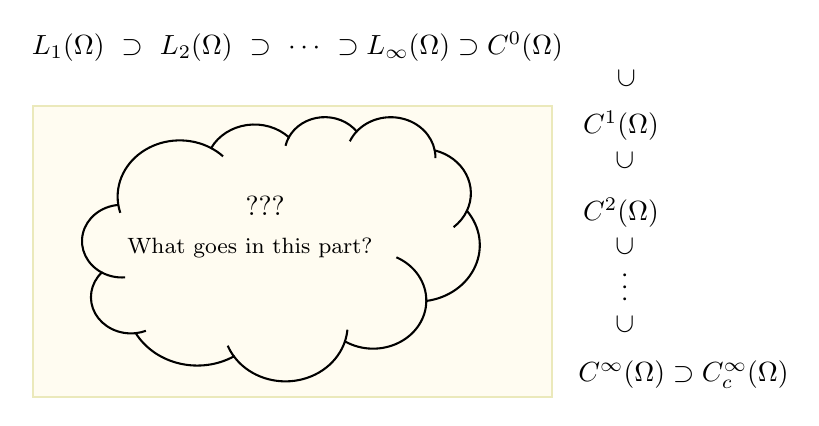
\begin{tikzpicture}[x=0.75pt,y=0.75pt,yscale=-1,xscale=1]
	%uncomment if require: \path (0,300); %set diagram left start at 0, and has height of 300
	
	%Shape: Rectangle [id:dp3131224415234657] 
	\draw  [color={rgb, 255:red, 235; green, 233; blue, 187 }  ,draw opacity=1 ][fill={rgb, 255:red, 255; green, 252; blue, 241 }  ,fill opacity=1 ] (120,90) -- (370,90) -- (370,230) -- (120,230) -- cycle ;
	%Shape: Cloud [id:dp6468787167291297] 
	\draw   (161.11,137.27) .. controls (159.56,127.01) and (164.63,116.84) .. (174.16,111.1) .. controls (183.69,105.35) and (196,105.03) .. (205.88,110.26) .. controls (209.38,104.29) and (215.79,100.18) .. (223.16,99.15) .. controls (230.54,98.12) and (238.01,100.31) .. (243.33,105.05) .. controls (246.31,99.64) and (252.16,96) .. (258.81,95.43) .. controls (265.46,94.86) and (271.96,97.44) .. (276.01,102.25) .. controls (281.4,96.51) and (289.97,94.1) .. (298.02,96.05) .. controls (306.06,98) and (312.13,103.96) .. (313.61,111.37) .. controls (320.21,113) and (325.71,117.14) .. (328.68,122.72) .. controls (331.66,128.3) and (331.81,134.78) .. (329.12,140.48) .. controls (335.62,148.14) and (337.14,158.34) .. (333.11,167.27) .. controls (329.09,176.21) and (320.12,182.55) .. (309.56,183.91) .. controls (309.49,192.3) and (304.41,200) .. (296.27,204.04) .. controls (288.14,208.08) and (278.23,207.83) .. (270.36,203.39) .. controls (267,213.43) and (257.57,220.83) .. (246.12,222.37) .. controls (234.68,223.91) and (223.28,219.33) .. (216.85,210.61) .. controls (208.97,214.91) and (199.51,216.15) .. (190.61,214.04) .. controls (181.71,211.94) and (174.12,206.67) .. (169.55,199.43) .. controls (161.5,200.28) and (153.71,196.51) .. (150.05,189.97) .. controls (146.4,183.44) and (147.65,175.54) .. (153.19,170.2) .. controls (146.01,166.37) and (142.34,158.78) .. (144.11,151.38) .. controls (145.87,143.98) and (152.66,138.45) .. (160.95,137.67) ; \draw   (153.19,170.2) .. controls (156.59,172.01) and (160.5,172.83) .. (164.42,172.55)(169.55,199.43) .. controls (171.23,199.25) and (172.88,198.87) .. (174.46,198.3)(216.85,210.61) .. controls (215.66,209) and (214.67,207.28) .. (213.89,205.48)(270.36,203.39) .. controls (270.97,201.55) and (271.36,199.67) .. (271.54,197.76)(309.56,183.91) .. controls (309.64,174.98) and (304.04,166.8) .. (295.16,162.89)(329.12,140.48) .. controls (327.68,143.52) and (325.48,146.22) .. (322.71,148.36)(313.61,111.37) .. controls (313.86,112.59) and (313.97,113.84) .. (313.95,115.09)(276.01,102.25) .. controls (274.67,103.68) and (273.57,105.28) .. (272.73,107)(243.33,105.05) .. controls (242.61,106.35) and (242.08,107.72) .. (241.74,109.15)(205.88,110.26) .. controls (207.97,111.37) and (209.91,112.71) .. (211.64,114.24)(161.11,137.27) .. controls (161.32,138.69) and (161.66,140.08) .. (162.11,141.45) ;
	
	% Text Node
	\draw (118,52.75) node [anchor=north west][inner sep=0.75pt]    {$L_{1}( \Omega ) \ \supset \ L_{2}( \Omega ) \ \supset \ \cdots \ \supset L_{\infty }( \Omega ) \supset C^{0}( \Omega )$};
	% Text Node
	\draw (411.27,70) node [anchor=north west][inner sep=0.75pt]  [rotate=-90]  {$\supset $};
	% Text Node
	\draw (383.67,90.73) node [anchor=north west][inner sep=0.75pt]    {$C^{1}( \Omega )$};
	% Text Node
	\draw (383.67,132.73) node [anchor=north west][inner sep=0.75pt]    {$C^{2}( \Omega )$};
	% Text Node
	\draw (410.6,109.33) node [anchor=north west][inner sep=0.75pt]  [rotate=-90]  {$\supset $};
	% Text Node
	\draw (381.33,211.07) node [anchor=north west][inner sep=0.75pt]    {$C^{\infty }( \Omega ) \supset C_{c}^{\infty }( \Omega )$};
	% Text Node
	\draw (410.6,151) node [anchor=north west][inner sep=0.75pt]  [rotate=-90]  {$\supset $};
	% Text Node
	\draw (409.27,168) node [anchor=north west][inner sep=0.75pt]  [rotate=-90]  {$\cdots $};
	% Text Node
	\draw (410.6,188.33) node [anchor=north west][inner sep=0.75pt]  [rotate=-90]  {$\supset $};
	% Text Node
	\draw (221,132) node [anchor=north west][inner sep=0.75pt]   [align=left] {???};
	% Text Node
	\draw (164,152) node [anchor=north west][inner sep=0.75pt]   [align=left] {{\footnotesize What goes in this part?}};
	
	
\end{tikzpicture}
\end{figure}
\FloatBarrier
\noindent Then the notion of the weak derivatives, and the Sobolev spaces come into play. We can define the notion of weak derivative for the functions that do not posses derivative in the classical sense, like the the function corresponding to the mapping $ x\mapsto \abs{x} $. 

For simplicity, we focus on the first derivative and try to generalize that notion. To do this, we need to focus on the set of functions that are continuously differentiable, i.e. $ \mathscr{C}^0(\Omega) $. Let $ f\in \mathscr{C}^0(\Omega) $. Then this function satisfies the following integration by parts identity
\[  \boxed{\int_\Omega f\ u'\ dx =  -\int_\Omega f'\ u\ dx, \qquad \forall u \in \mathscr{C}^\infty_c(\Omega).} \]
Where $ \mathscr{C}^\infty_c(\Omega) $ is the set of all smooth functions with compact support. The identity above holds because
\[  \int_\Omega f\ u'\ dx  = \underbrace{\big[f\ u\big]_{\partial \Omega}}_{0}-\int_\Omega f'\ u\ dx . \]
Note that the boundary above is zero since the function $ u $ has compact support, thus it is zero at the boundary. Now using this identity, we can extend the notion of derivatives to the functions that do not posses derivatives in the classic sense. This is the intuitive idea behind the notion of Sobolev spaces. 

\begin{definition}[Sobolev Spaces]
	Let $ \Omega\subset \R^n $. Then we define $ W^{k,p} $ to be the space of functions in $ L_p(\Omega) $ that posses $ k $ weak derivatives that belong to $ L_p(\Omega) $. In other words, for $ k $ a non-negative integer, we have
	\[ W^{k,p} = \Set{u\in L_p(\Omega)\ :\  u_\alpha \in L_p(\Omega),\ \abs{\alpha} \leq k }, \]
	Where $ u_\alpha $ defined to be
	\[  u_\alpha = v \quad \Longleftrightarrow \quad \int_\Omega u\ D^\alpha f\ dx = (-1)^{\abs{\alpha}} \int_\Omega v f \ dx, \quad \forall f \in \mathscr{C}^\infty_c(\Omega). \]
	Or in a more compact notation we can write
	\[ u_\alpha = v \quad  \Longleftrightarrow \quad (u,D^\alpha f) = (v,f). \]
	So we can use the following equivalent definition for the Sobolev spaces.
	\[ W^{k,p} = \Set{u \in L_p(\Omega)\ :\ \exists v \in L_p(\Omega) \st (u,D^\alpha f) = (v,f) \quad \forall f \in \mathscr{C}^\infty_c(\Omega)}. \]
	Note that we sometimes, when there is not ambiguity, we denote the weak derivative of $ u $ with $ u_\alpha $ and $ D^\alpha u $ interchangeably.
\end{definition}

\begin{beCareful}
	Consider the following definition of $ W^{k,p} $
	\[ W^{k,p} = \Set{u \in L_p(\Omega)\ :\ \exists v \in L_p(\Omega) \st (u,D^\alpha f) = (v,f) \quad \forall f \in \mathscr{C}^\infty_c(\Omega)}. \]
	A careful reader might raise the question that how does one know that the integral $ (u, D^\alpha f) $ exists given $ u \in L_p(\Omega) $ and $ D^\alpha f \in \mathscr{C}^\infty_c(\Omega) $? To show this we utilize the H\"{o}lder's inequality. First, observe that $ \mathscr{C}^\infty_c(\Omega) \subset L_p(\Omega)$ for all $ p\geq 1 $, and in particular $ \mathscr{C}^\infty_c(\Omega) \subset L_q(\Omega) $ where $ 1/q = 1-1/p $. Thus using the H\"{o}lder's inequality we can write
	\[ (u, D^\alpha f) = \int_\Omega \abs{u\ D^\alpha f}\ dx \leq \norm{u}_{L_p} \norm{D^\alpha f}_{L_q} < \infty. \]
\end{beCareful}


The following proposition shows that the Sobolev spaces are actually normed vector spaces.

\begin{theorem}[Sobolev spaces are normed vector spaces]
	Let $ \Omega \subset \R^n $. Then $ (W^{k,p}(\Omega), \norm{\cdot}_{W^{k,p}(\Omega)}) $ is a normed vector space. For $ u \in W^{k,p}(\Omega) $ we have
	\[  \norm{u}_{W^{k,p}(\Omega)} = \big(\sum_{\abs{\alpha}\leq k}\norm{D^\alpha u}^p_{L_p(\Omega)}\big)^{1/p}.  \]
	Also we define the semi-norm (this is semi-norm since it is not positive definite) as
	\[ \abs{u}_{W^{k,p}(\Omega)} = \big(\sum_{\abs{\alpha} =  k}\norm{D^\alpha u}^p_{L_p(\Omega)}\big)^{1/p}.\]
	Thus the norm can be written as 
	\[ \norm{u}_{W^{k,p}(\Omega)} = \big( \sum_{i=1}^{k}\abs{u}^p_{W^{i,p}(\Omega)} \big)^{1/p}. \]
\end{theorem}
For the special case where $ p=2 $, the Sobolev space $ W^{k,2}(\Omega) $ will have more interesting features as summarized bellow.

\begin{proposition}[$ W^{k,2}(\Omega) $ is a Hilbert space]
	Let $ \Omega \subset \R^n $. Then $ W^{k,2}(\Omega) $ is a Hilbert space with the following inner product
	\[ (u,v)_{W^{k,2}(\Omega)} = \sum_{\abs{\alpha}\leq k}(D^\alpha u, D^\alpha v). \]
	We usually denote this space as
	\[  H^k := W^{k,2}(\Omega). \]
\end{proposition}

The definitions and notations above are for the general setting. However, throughout this notes we will mostly be working with $ H_1(\Omega) $ and $ H^2(\Omega) $. So in the following example we will go through the definitions for these special cases to train our eye for those notations.

\begin{example}[Special cases of Sobolev spaces]
	Let $ \Omega \subset \R^n $. Then $ H^1(\Omega) $ and $ H^2(\Omega) $ are the set of all square integrable functions that posses first and second weak derivatives respectively.\\
	We start with $ H^1(\Omega) $ which is defined to be
	\[ H^1(\Omega) = \Set{f\in L_2(\Omega)\ :\ \big(\frac{\partial f}{\partial x_i}\big) \in L_2(\Omega),\ i=1,2,\cdots,n },\]
	\[ \norm{u}_{H^1(\Omega)} = \big(\norm{f}^2_{L_2(\Omega)} + \sum_{i=1}^{n}\norm{\frac{\partial f}{\partial x_i}}_{L_2(\Omega)}^2\big)^{1/2}, \] 
	\[ \abs{u}_{H^1(\Omega)} = \big(\sum_{i=1}^{n}\norm{\frac{\partial f}{\partial x_i}}_{L_2(\Omega)}^2\big)^{1/2} \]
	
	Similarly, for $ H^2(\Omega) $ we can write
	\begin{align*}
		H^2(\Omega) = &\{ f:\Omega \to \mathbb{R}\ : (\frac{\partial f}{\partial x_i}) \in L_2(\Omega),\ i=1,2,\ldots,n, \nonumber \\
		&\phantom{{}= \{ f:\Omega \to \mathbb{R}\ :} (\frac{\partial^2 f}{\partial x_i \partial x_j}) \in L_2(\Omega),\ i,j=1,2,\ldots,n \}.
	\end{align*}
	\[ \norm{u}_{H^2(\Omega)} = \big( \norm{u}^2_{L_2(\Omega)} + \sum_{i=1}^{n} \norm{\frac{\partial f}{\partial x_i}}^2_{L_2(\Omega)}  + \sum_{i,j=1}^{n} \norm{\frac{\partial^2 f}{\partial x_i \partial x_j}}_{L_2(\Omega)}\big)^{1/2}, \]
	and for the semi-norm we have
	\[ \abs{u}_{H^2(\Omega)} = \big(\sum_{i,j=1}^{n} \norm{\frac{\partial^2 f}{\partial x_i \partial x_j}}_{L_2(\Omega)}\big)^{1/2}. \]
\end{example}

The following definition introduces an important special Sobolev space.

\begin{definition}[Definition of $ H_0^1(\Omega) $]
	The Sobolev space $ H_0^1(\Omega) $ is defined to be the closure of $ \mathscr{C}^\infty_c(\Omega) $ under $ \norm{\cdot}_{H^1(\Omega)} $ norm. I.e. for any sequence $ \set{u_n} $ in $ \mathscr{C}^\infty_c(\Omega) $ that converges to $ u^* $ under $ \norm{\cdot}_{H^1(\Omega)} $, then $ u^* \in H_0^1 $.
\end{definition}
\begin{remark}
	For instance, Let $ \Omega = [-1,1] $. Then the following function is in $ H^1_0(\Omega) $.
	\[ 
	f(x) = \begin{cases}
		1-\abs{x} \qquad &x\in[-1/2,1/2],\\
		0 \qquad &\text{else}.
	\end{cases}
	 \]
\end{remark}

The following proposition gives us some intuitive characterization of $ H^1_0(\Omega) $.

\begin{proposition}
	Let $ \Omega \subset\R^n $ an open set with a sufficiently smooth boundary. Then 
	\[ H_0^1(\Omega) = \Set{f \in H^1(\Omega)\ :\ f(\partial \Omega) = 0}.   \]
\end{proposition}

We conclude this section with the important inequality of Poincar\'{e}-Friedrichs inequality.

\begin{theorem}[Poincar\'{e}-Friedrichs inequality]
	Let $ \Omega \subset \R^n $. Then $ \exists C_{\star} \in \R $ that depends on the geometry of the domain $ \Omega $ and for all $ u \in H_0^1(\Omega) $ we have
	\[ \int_\Omega \abs{u(x)}^2\ dx \leq  C_{\star} \sum_{i=1}^{n} \int_\Omega \Abs{\frac{\partial u}{\partial x_i}}^2\ dx, \qquad \forall u \in H_0^1. \]
	Or equivalently we can write this in a more compact notation as follows
	\[ \norm{u}_{L_2(\Omega)} \leq \tilde{C_{\star}} \abs{u}_{H^1}. \]
\end{theorem}
\begin{proof}
	To demonstrate the simplicity of the proof for such an un-intuitive result, we start with assuming $ \Omega = [a,b] \subset \R $. Let $ u \in H^1_0(\Omega) $. Then we can write
	\[ u(x) = u(a) + \int_{a}^{x}u'(\xi)\ d\xi = \int_{a}^{x}u'(\xi)\ d\xi, \qquad a\leq x\leq b \]
	Note that since $ u \in H_0^1(\Omega) $, then $ u $ is zero at the boundary. Now we can write
	\[ \int_{a}^{b} \abs{u(x)}^2 dx = \int_{a}^{b}\abs{\int_{a}^{x}u'(\xi)\ d\xi}^2 d\xi. \]
	We can simplify the inner integral using the Cauchy-Schwartz inequality
	\[ \int_{a}^{x} u'(\xi)\ d\xi \leq (x-a)^{1/2}(\int_{a}^{x}\abs{u'(\xi)}^2\ d\xi)^{1/2} \]
	Also, note that we can write
	\[ \int_{a}^{x} \abs{u'(\xi)}^2\ d\xi \leq \int_{a}^{b}\abs{u'(\xi)}^2\ d\xi.  \]
	This is true since the integrand is always positive. Putting the pieces together we can not write
	\[ \int_{a}^{b} \abs{u(x)}^2 dx = \int_{a}^{b}\abs{\int_{a}^{x}u'(\xi)\ d\xi}^2 d\xi \leq \frac{(b-a)^2}{2} \int_{a}^{b}\abs{u'(\xi)}^2\ d\xi. \]
	
	For another simple case $ \Omega = [a,b]\times [c,d] \subset \R^2 $, the proof will be pretty much analogous to the proof above, with a difference that we will need to find an upper bound for $\int_{a}^{b}\int_{c}^{d}\abs{u(x,y)}^2dydx$ twice (one with respect to the $ u_x $ and the other one with respect to $ u_y $). Also, note that we will need to use the identity that for every $ a,b >0 $, $ ab/(a+b) $ is an upper bound for both $ a $ and $ b $. Eventually we can show that 
	\[ \int_{\Omega} \abs{u(x,y)}^2\ dxdy \leq \underbrace{(\frac{2}{(d-c)^2} + \frac{2}{(b-a)^2})^{-1}}_{C_\star}\int_\Omega (\abs{u_x}^2 + \abs{u_y}^2) dxdy \]
\end{proof}

\begin{example}
	Let $ \Omega = [0,1]\times [0,1] \subset \R^2$. Then we have
	\[ \int_\Omega\abs{u(x,y)}^2 dxdy \leq \frac{1}{4} \int_\Omega (\abs{u_x(x,y)}^2 + \abs{u_y(x,y)}^2)\ dxdy \qquad \forall u \in H_0^1(\Omega) \]
\end{example}

\begin{example}
	Let $ \Omega = [0,1] \subset \R $. Then we have
	\[ \int_\Omega\abs{u(x,y)}^2 dx \leq \frac{1}{2} \int_\Omega \abs{u_x(x,y)}^2 \ dx \qquad \forall u \in H_0^1(\Omega) \]
\end{example}





\section{PDEs and the Weak Solutions}



\section{Working Area}
Things to add: Example for weak derivative, completing the diagram for the geometry of the function spaces. 